% 设定文章类型,正文字号为小四,若为五号将-4改为5即可
\documentclass[zihao=-4,UTF8]{report}		

% 导入基本宏包
\usepackage[UTF8]{ctex}       % 设置文档为中文语言(中文paper留此行,删去上一行)
\usepackage{amsmath}    % 宏包:数学公式
\usepackage{amssymb}    % 宏包:提供更多数学符号
\usepackage{pifont}     % 宏包:提供了特殊符号和字体
\usepackage{extarrows}  % 宏包:更多箭头符号
\usepackage{hyperref}	% 宏包:添加超链接

%宏包:有色文本框及其设置
\usepackage[dvipsnames,svgnames]{xcolor}    %设置插入的文本框颜色
\usepackage[strict]{changepage}     % 提供一个 adjustwidth 环境
\usepackage{framed}     % 实现方框效果
\definecolor{graybox_color}{rgb}{0.95,0.95,0.96} % 文本框颜色。修改此行中的 rgb 数值即可改变方框纹颜色,具体颜色的rgb数值可以在网站https://colordrop.io/中获得。(截止目前的尝试还没有成功过,感觉单位不一样)(找到喜欢的颜色,点击下方的小眼睛,找到rgb值,复制修改即可)
\newenvironment{graybox}{%
\def\FrameCommand{%
\hspace{1pt}%
{\color{gray}\vrule width 2pt}%
{\color{graybox_color}\vrule width 4pt}%
\colorbox{graybox_color}%
}%
\MakeFramed{\advance\hsize-\width\FrameRestore}%
\noindent\hspace{-4.55pt}% disable indenting first paragraph
\begin{adjustwidth}{}{7pt}%
\vspace{2pt}\vspace{2pt}%
}
{%
\vspace{2pt}\end{adjustwidth}\endMakeFramed%
}

% 文章页面margin设置
\usepackage[a4paper]{geometry}
\geometry{top=1in}
\geometry{bottom=1in}
\geometry{left=0.75in}
\geometry{right=0.75in}   % 设置上下左右页边距
\geometry{marginparwidth=1.75cm}    % 设置边注距离(注释、标记等)

% 标题自定义设置
\usepackage{titling}  % 宏包:标题设置

% 表格进阶设置
\usepackage{booktabs}
\usepackage{tabularx}
\usepackage{array}
\usepackage{longtable}
\usepackage{multirow}
\usepackage{tabularray}

% 图表插入自定义设置
\usepackage{graphicx}  % 宏包:图片插入
\usepackage{float}     
\usepackage{caption}
\captionsetup[figure]{name=图}  % 设置图标题为“图”以防出现“figure”
\captionsetup[table]{name=表}   % 设置表标题为“表”以防出现“table”
\captionsetup{labelfont=bf, font=small}   % 将表、图等标题设置为bf,字号为small(五号)
\usepackage[export]{adjustbox}               

% 文章默认字体设置
\usepackage{fontspec}   % 宏包:更多字体种类
\usepackage{xcolor}    % 宏包:更多颜色设置
\setmainfont{SimSun}    % 设置中文字体为宋体字体
\setmainfont{Times New Roman} % 设置英文字体为Times New Roman

% 参考文献引用设置
\bibliographystyle{unsrt}   % 设置参考文献引用格式为unsrt
\newcommand{\upcite}[1]{ {\cite{#1}}}     % 自定义上角标式引用

% chapter标题自定义设置
\usepackage{titlesec}   
\titleformat{\chapter}[hang]{\normalfont\huge\bfseries\centering}{第\,\thechapter\,章}{20pt}{\Huge}
\titlespacing*{\chapter}{0pt}{-15pt}{20pt} % 控制上方空白的大小


% 文章序言设置
\newcommand{\enabstractname}{Abstract}
\newcommand{\cnabstractname}{序言}
\newenvironment{enabstract}{%
  \par\Large
  \noindent\mbox{}\hfill{\bfseries \enabstractname}\hfill\mbox{}\par
  \vskip 2.5ex}{\par\vskip 2.5ex}
\newenvironment{cnabstract}{%
  \par\Large
  \noindent\mbox{}\hfill{\bfseries \cnabstractname}\hfill\mbox{}\par
  \vskip 2.5ex}{\par\vskip 2.5ex}

  % 页眉页脚设置
\usepackage{fancyhdr}   %宏包:页眉页脚设置
\pagestyle{fancy}
\fancyhf{}
\cfoot{\thepage}
\renewcommand\headrulewidth{1pt}
\renewcommand\footrulewidth{0pt}
\chead{The Notes of Combined Programming Language}    

% 文档作者信息设置
\title{\textbf{C语言笔记\\The Notes of Combined Programming Language}}
\author{丁毅\\ \footnotesize 中国科学院大学,北京 100049\\ Yi Ding \\ \footnotesize University of Chinese Academy of Sciences, Beijing 100049, China}
\date{\footnotesize 2024.3.18—}

% 外源代码插入设置
\newfontfamily\TimesNR{Times New Roman}
\usepackage{listings}
\lstset{
    language=C,
    basicstyle=\linespread{1.1}\small\setmainfont{Consolas},
    keywordstyle=\color{blue},
    stringstyle=\color{red},
    commentstyle=\color{green!70!black}\normalfont,
    morecomment=[l][\color{gray!70}]{\#},
    showstringspaces=false,
    numbers=left,
    numberstyle=\small,
    numbersep=10pt,
    tabsize=2,
    breaklines=true,
    breakatwhitespace=true,
    frame=single,
    framesep=0.25em, % 设置边框与代码的距离
    title=\lstname,
    captionpos=b,
    belowskip=-14pt,
    aboveskip=12pt,
    xleftmargin=2em, %整体距左侧边线的距离为2em
    xrightmargin=2em, %整体距右侧边线的距离为2em
    columns=flexible,
}

 % 开始编辑文章
 \begin{document}
 \maketitle
 \newpage
 
 \addcontentsline{toc}{chapter}{序言} %手动添加为目录
 \thispagestyle{fancy}   %显示页码、页眉等
 \begin{cnabstract}
 {\normalsize 本书是笔者本科时的C语言学习笔记,总结了C语言学习中的主要知识,也有适当的拓展延伸。同时,对一些晦涩的概念,给出了笔者的个人理解,以帮助读者阅读。}
 \end{cnabstract}
 \pagenumbering{Roman} %页码为大写罗马数字
 
 \newpage
 \addcontentsline{toc}{chapter}{目录}
 \tableofcontents
 \thispagestyle{fancy}
 
 \newpage
 \pagenumbering{arabic} 

\chapter{基础知识}
\section{C语言概述}
\subsubsection{学习语言的第一步\  ——\ Hello world:}
你好你好
\begin{lstlisting}[caption={Hello world!}]
#include <stdio.h>
int main()
{
    printf("Hello, world!\n");
    return 0;
}
\end{lstlisting}
\subsubsection{main函数:}
main称为主函数,C语言程序是从主函数的第一行开始执行的,一个项目可以有多个.c文件,但仅能有一个main函数。
{\color{gray} $
1\ \text{bit} = 1\ \text{b} \overset{\times 8 }{\longrightarrow } 1 \ \text{byte} = 1 \ \text{B} \overset{\times 1024 }{\longrightarrow }1 \ \text{KB} \overset{\times 1024 }{\longrightarrow }1 \ \text{MB} \overset{\times 1024 }{\longrightarrow }1 \ \text{GB}\overset{\times 1024 }{\longrightarrow }1 \ \text{TB}\overset{\times 1024 }{\longrightarrow }1 \ \text{PB}
$}

\subsubsection{较完整的C程序(计算长方体体积):}
\begin{lstlisting}
#include <stdio.h>  
#define h 10    
/*
引入库stdio.h
利用“宏”定义h,起替换作用
*/
int solve(int x, int y);  //函数声明(必要的)
int main()
{
    system("color f3");
    int x, y, v;
    printf("长方体高度为:%d\n", h);
    printf("请输入长方体的长和宽:\n");
    scanf_s("%d %d", &x, &y);
    v = solve(x, y);
    printf("长方体的体积是%d\n", v);
    return 0;
}   
int solve(int x, int y)     //定义函数solve
{
    int v = h * x * y;
    return v;
}
\end{lstlisting}\noindent

\section{算法}
算法,即使用计算机解决问题的方法。优秀的算法应具有正确性、可读性、健壮性、较低的时间复杂度与空间复杂度。我们常用流程图等方法帮助构建算法。

\section{数据类型}
\subsubsection{命名规范:}
\ding{172}\ 常量:常量命名统一为大写格式。{\color{gray} \#define AGE 28 }\par
\ding{173}\ 变量:如果是成员变量,均以m\_开始。如果是普通变量,取与实际意义相关的名称,并且名称的首字母要大写,再在前面添加类型的首字母。{\color{gray} int m\_age; \ \  int number; }\par\par
\ding{174}\ 指针:在标识符前添加p字符,并且名称首字母要大写。{\color{gray} int * pAge;}\par
\ding{175}\ 函数:定义函数时,函数名的首字母要大写,其后的字母根据含义大小写混合。

\subsubsection{关键字:}
关键字(Keywords),又称为保留字,是C语言规定的具有特定意义的字符串。用户定义的常量、变量、函数等名称不能与关键字相同,否则会出现错误。

\subsubsection{标识符:}
变量、常量、函数、数组等的名称就是所谓的标识符。\par
\ding{172}\ 标识符必须以字母或下画线开头,而不能以数字或者符号开
头。\par
\ding{173}\ 标识符中,除开头外的其他字符可以由字母、下画线或数字组
成。\par
\ding{174}\ 区分大小写,不能是关键字,应体现一定的功能含义。\par

\subsubsection{变量的储存类别:}
变量的储存类别有auto,static,register,extern四种。auto相当于自定义函数中的局部变量,static相当于全局变量,例如``static int x = 3"定义了一个static的整型变量(初始值为3)。
\subsubsection{数据类型:}
数据类型可分为基本类型、构造类型、指针类型和空类型。C语言中,整数的默认类型是int,浮点数的默认类型是double,如果一个表达式中数字都是int型,则表达式结果也默认为是int型。要特别注意,两个整数作除法时,要将其中之一转为float,否则输出int。
\subsubsection{强制类型转换:}
如果某个表达式要进行强制类型转换,需要将该表达式用括号括起来,否则将只对表达式中的第一个变量或常量进行强制类型转换。语法如下:
\begin{lstlisting}
*** = (类型)  (变量/表达式)

例如:
    float y = 5.0/3; 
    int z = (int) y;    //结果:z=1(int型)
    float j = (float) (z+y) + y;    //结果:j=4.333(float型)


\end{lstlisting}

\begin{table}[H]
    \caption{\textbf{数据类型中的基本类型}}
    \centering
    \begin{tabular}{cccc} 
    \toprule
    类型     & 关键字             & 字节 & 数值范围  \\
    \hline
    短整型    & short~          & 2    & $[-2^{15},\ 2^{15}-1]$      \\
    无符号短整型 & unsigned short~ & 2 &  $[0,\ 2^{16}-1]$    \\
    整型     & ~int            & 4     &  -   \\
    无符号整型  & unsigned~       & 4  &   - \\
    长整型    & long            & 4    &    -   \\
    无符号长整型 & unsigned long   & 4 &     -  \\
    单精度浮点  & float           & 1  &     $[-3.4\times 10^{-38},\ 3.4\times 10^{38}]$  \\
    双精度浮点  &  double & 1  &     $[-1.7\times 10^{-308},\ 3.4\times 10^{308}]$ \\
    长双精度浮点 & long double          & 4 &      - \\
    字符型    & char       & 8   &      $[-128,\  127]$ \\
    无符号字符型 & unsigned char     & 8 &      $[0,\ 256]$ \\
    \bottomrule
    \end{tabular}
\end{table}

\subsubsection{转义字符:}
\begin{table}[H]
    \centering
    \caption{\textbf{常见转义字符}}
    \begin{tabular}{cccc} 
    \toprule
     {转义字符}              &  {意义}       &  {转义字符}                                                 &  {意义}                                     \\ 
    \hline
     {\textbackslash{}n} &  {回车换行}     &  {\textbackslash{}\textbackslash{}}                     &  {反斜杠\textbackslash{}}                  \\
     {\textbackslash{}t} &  {Tab键横向跳跃} &  {\textbackslash{}'}                                    &  {单引号符}                                   \\
     {\textbackslash{}v} &  {竖向跳格}     &  {\textbackslash{}a}                                    &  {alarm鸣铃}                                \\
     {\textbackslash{}b} &  {退格}       & {\textbackslash{}f} &  {换页}  \\
     {\textbackslash{}r} &  {回车}       &                                                                        &                                                          \\
    \bottomrule
    \end{tabular}
\end{table}

\section{运算符}
\subsubsection{运算符:}
运算符分为赋值运算符、算术运算符、关系运算符、逻辑运算符、位逻辑运算符、逗号运算符、复合赋值运算符等。在使用运算符时,要特别注意各个运算符之间的优先级。
\begin{table}[H]
    \centering
    \caption{\textbf{部分运算符}}
    \begin{tabular}{ccccc} 
    \toprule
    运算符 & 名称     & 功能                 & 示例        & \multicolumn{1}{l}{结果}  \\
    \hline
    \textbackslash & 除法运算符  & 除法                 & 5/2       & 2      \\
    \%  & 求余运算符  & 求余                 & 5\%2      & 1      \\
    +\,+  & 自增运算符  & 使变量增加1(不能用于常量、表达式) & 1+\,+;\ ++1       & 1; 2      \\
    -\,-  & 自减运算符  & 使变量减少1(不能用于常量、表达式) & 1-\,-; -\,-1        &  1; 0       \\
    \&\&   & 逻辑与运算符 & 与                  & 1<0 \&\& 2>1      & 1      \\
    ||    & 逻辑或运算符 & 或                  & 1==0 || 2>1 & 1       \\
    !   & 逻辑非运算符 & 非                  & !1==0     & 1      \\
    \bottomrule
    \end{tabular}
\end{table}
特别地,对于自增符:A+\,+表示先输出A,再执行A = A+1,+\,+A表示先执行A = A+1,再输出A。自减运算符类似。
\subsubsection{逗号表达式:}
逗号表达式又称为顺序求值运算符,其求解过程是:先求解表达式1,再求解表达式2,一直求解到表达式n。整个逗号表达式的值是表达式n的值。
\begin{lstlisting}
(表达式1, 表达式2, ... , 表达式n)

例如:
((1+2, 3), 9)        //结果:9

int x=3, y=3, z=1;
printf("%d,%d",(++x,y++),z+x+y+2)          //结果:3, 10
\end{lstlisting}\par
逗号表达式又称为顺序求值运算符,其求解过程是:先求解表达式1,再求解表达式2,一直求解到表达式n。整个逗号表达式的值是表达式n的值。

\section{数据输入与输出}
\subsubsection{常用数据输入/输出函数:}
常见数据输入/输出函数如下表:

\begin{table}[H]
    \centering
    \caption{\textbf{常见数据输入/输出函数}}
    \begin{tabular}{cccc}
    \toprule
    函数        & 名称      & 例子& 结果 \\
    \hline
    putchar() & 字符输出函数  & putchar('a')& a \\
    \hline
    getchar() & 字符输入函数  & \begin{tabular}[c]{@{}l@{}}char x = getchar();\\ putchar(x);\end{tabular}   & \begin{tabular}[c]{@{}l@{}}(键盘上输入a)\\ a\end{tabular} \\
    \hline
    puts()    & 字符串输出函数 & puts("Love You")   & Love You        \\
    \hline
    gets()    & 字符串输入函数 & \begin{tabular}[c]{@{}l@{}}char password[20];\\ gets(password);\\ puts("确认你的密码是:");\\ puts(password);\end{tabular}     & \begin{tabular}[c]{@{}l@{}}(键盘上输入123)\\ 123\end{tabular}    \\
    \hline
    printf()  & 格式输出函数  & \begin{tabular}[c]{@{}l@{}}int x = 1;\\ 	printf("今年她\%d岁了。", x);\end{tabular}   & 今年她1岁了。  \\
    \hline
    scanf()   & 格式输入函数  & \begin{tabular}[c]{@{}l@{}}~~~ char str[100];\\ printf("请输入一个字符串:");\\ scanf\_s("\%s", \textcolor{red}{\&}str);\\ printf("输入的字符串是:\%s\textbackslash{}n", str);\end{tabular} & \begin{tabular}[c]{@{}l@{}}请输入一个字符串:\\ (键盘上输入dddk)\\ 输入的字符串是:dddk\end{tabular} \\
    \bottomrule
    \end{tabular}
\end{table}

\noindent 注:\par
puts函数识别到结束符 \textbackslash 0 时,后面的字符不再输出,并且自动换行(编译器会自动在字符串末尾添加结束符 \textbackslash 0)\par
printf函数格式控制字符见表。\par
scanf函数格式控制字符见表。特别注意scanf函数的第二个参数是变量地址,而不是变量标识符,勿忘加上\textcolor{red}{\&}。另外,在Visual Studio 2022中,scanf函数无法使用,解决方法是将所有的scanf函数替换为scanf\_s函数,就如表中的例子一样。
\begin{table}[H]
    \centering
    \caption{\textbf{printf, scanf格式控制字符}}
    \begin{tabular}{ccc} 
    \toprule
    类型              & prinft格式字符 & scanf格式字符  \\
    有符号整数           & \%d, \%i   & \%d, \%i   \\
    无符号整数           & \%u        & \%u        \\
    浮点数(小数形式)       & \%f        & \%f        \\
    ~浮点数(指数形式)      & \%e        & \%e        \\
    \%f和\%e中宽度较短的形式 & \%g        & \%g        \\
    无符号八进制整数        & \%o        & \%o        \\
    无符号十六进制整数       & \%x        & \%x        \\
    单个字符            & \%c        & \%c        \\
    字符串             & \%s        & \%s        \\
    \bottomrule
    \end{tabular}
    \end{table}

\section{条件语句}
\subsubsection{常见条件语句:}
\ding{172}\ if, else if, else语句:\par
语法如下:
\begin{lstlisting}
if(){代码}
else if(){代码}
else(){代码}
\end{lstlisting}

\ding{173}\ 条件运算符\ ` ? '  :\par
检验第一个表达式的真假,并根据检验结果返回第二、三个表达式的其中一个。语法如下:
\begin{lstlisting}
表达式1?表达式2:表达式3

例如:
x = (3>2)?50:10; 
printf("%d", x);    //结果:50
\end{lstlisting}\par
\ding{174}\ switch语句:\par
计算表达式的值,与case中的常量/常量表达式进行比较(不可为变量),执行符合情况的语句,如果没有情况符合,执行default语句(可以省略)。语法如下:
\begin{lstlisting}
swich(条件)
{
    case 1:
        情况1的代码;
    case 2:
        情况2的代码;
    case 3:
    case 4:
        情况3和4的代码
    default:
        代码;
}
\end{lstlisting}

\section{循环控制}
\subsubsection{循环语句:}
\ding{172}\ while语句:\par
语法如下:
\begin{lstlisting}
while(条件){代码}

例如:
int n = 0;
scanf_s("%i", &n);
while (n <= 100) 
{
    printf("%i;", n++);
}
printf("%i", n);
/*结果(键盘中输入70):
70;71;72;73;74;75;76;77;78;79;80;81;82;83;84;85;
86;87;88;89;90;91;92;93;94;95;96;97;98;99;100;101
*/
\end{lstlisting}
\ding{173}\ do ... while语句:\par
在有些情况下,不论条件是否满足,循环过程必须执行至少一次,语法如下:
\begin{lstlisting}
do{代码}while(条件);     //例子懒得给了
\end{lstlisting}
\ding{174}\ for语句:\par
for语句首先计算第1个表达式的值,接着计算第2个表达式的值。如果第2个表达式的值为真,程序就执行循环体的内容,并计算第3个表达式;然后检验第2个表达式,执行循环;如此反复,直到第2个表达式的值为假,退出循环。语法如下:
\begin{lstlisting}
for(表达式; 条件; 表达式;){代码}
我们常把其写为:
for(循环变量赋初值; 循环条件; 循环变量改变;){代码} 
//赋初值一处可以利用逗号语句赋给多个变量初值
\end{lstlisting}
\ding{175}\ 循环嵌套:略。

\subsubsection{转移语句:}
\ding{172}\ goto语句:\par
使程序立即跳转到函数内部的任意一条可执行语句处。标识符要在程序的其他
位置给出,并且标识符要位于函数内部。语法如下:
\begin{lstlisting}
goto 标识符;

例如:
goto Show;
printf("我是小明");
Show:
    printf("我是小蓝");
/*结果:
我是小蓝
*/
\end{lstlisting}\par

\ding{173}\ break语句:\par
用于终止并跳出当前循环,然后继续执行后面的代码。语法略。\par
\ding{174}\ continue语句:\par
结束本次循环,即跳过循环体中尚未执行的部分,直接执行下一次的循环操作。语法略。

\chapter{核心内容}

\section{函数}
\subsubsection{函数的定义:}
定义函数的语法如下:
\begin{lstlisting}
/*声明函数(分号结尾。如果先定义函数,再调用函数,则不需要进行函数声明)*/
返回值类型 函数名(参数1, 参数2, ...); 
/*定义函数(函数参数可以是常量、变量、数组、指针等,也可以是表达式)*/
返回值类型 函数名(参数1, 参数2, ...)   
{
    函数体
}
\end{lstlisting}
另外,函数在编译时会被分配一个入口地址,因此指针变量也可以指向一个函数,通过该指针变量调用此函数。\par
\subsubsection{外部函数与内部函数:}
外部函数是可以被其他源文件调用的函数,内部函数(又称静态函数)只能被所在的源文件使用。不加其它说明的函数即为外部函数,内部函数语法如下:
\begin{lstlisting}
static 返回值类型 函数名(参数列表)
\end{lstlisting}
{\color{gray}\small 使用内部函数的好处是,不同开发者编写函数时,不必再担心函数是否会与其他源文件中的函数同名。因为内部函数只在所在源文件中有效,不同源文件中即使有相同的函数名,也没有关系。}


\section{数组}
\subsubsection{数组定义及引用:}
数组实际上是一组相同类型数据的集合(可理解为矩阵)。数组定义及引用的例子:
\begin{lstlisting}
int array1[5] = {666,888,999};
int array2[3][5] = {{10,20,30,40,50},{100}};
printf("%d %d\n", array1[0],array1[1]);
printf("%d", array2[0][3]);
/*结果:
666 888
40
*/
\end{lstlisting}
得到的数组分别为:
\begin{equation*}
    \text{array1} = 
    \begin{bmatrix}
        666&888&999&0&0
    \end{bmatrix}\ ,\ \ 
    \text{array2} = 
    \begin{bmatrix}
       10& 20 & 30 & 40 & 50\\
       100 & 0 & 0 & 0 & 0\\
       0 & 0 & 0 & 0 & 0
    \end{bmatrix}
\end{equation*}\par
特别注意,与其它编程语言类似,数组的序号索引是从0开始的。{\color{gray}\small 为避免混淆,在引用第$i$行$j$列的元素时,可以采用$\text{array}[i-1][j-1]$的形式。下标错误的常见报错为“C6385	正在从 array2 读取无效数据”与“C6201	索引5超出了0至2的有效范围”。}\par
特别地,对于字符数组:
\begin{lstlisting}
char c_array[] = {"love"};    //使用字符数组保存字符串时,系统会自动为其添加“\0”作为结束符。
char c_array[] = "love";    //用字符串进行赋值时可以去掉大括号
\end{lstlisting}
得到的字符数组实际为:
\begin{equation*}
    \text{c\_array} =[\,  \text{l}\ \text{o}\ \text{v}\ \text{e}\ \text{\textbackslash 0}\, ]
\end{equation*}\par
\subsubsection{数组名到底是什么:}
数组名本质上是地址和值相同的特殊指针常量,实际运用时可视作{\color{red}(指向首元素地址的)普通指针常量。}{\color{gray}\small 指针常量:其值不可修改的指针。只有在两种场合下(sizeof函数和\&操作符,即设计到数组大小或数组名地址时),数组名不能视为指针常量,其他场合可完全等价使用。}\par
一维数组的例子:\par
\ding{172}\ a是int型指针常量(a的类型int * ,值不可修改,a的元素类型是int)\par
\ding{173}\ a的地址(\&a) = a的值(a) = 首地址(首元素地址)
\begin{lstlisting}
int a[3] = {1,2,3};     
printf("a的值是:%p",a);
printf("a[0]的地址是:%p",a);
printf("a[0]的值是:%p",a[0]);

a的值是:000000B1D24FF618
a[0]的地址是:000000B1D24FF618
a[0]的值是:1
\end{lstlisting}\par
二维数组的例子:\par
\ding{172}\ a是(int*)型指针常量(a的类型int ** ,值不可修改,a的元素类型是int*)
\par
\ding{173}\ a的地址(\&a) = a的值(a) = 首地址(首元素地址)
\begin{lstlisting}
int a[2][3] = { {1,2,3},{4,5,6} };
printf("a的值是:%p\n", a);
printf("a[0]的地址是:%p\n", &a[0]);
printf("a[0]的值是:%p\n", a[0]);
printf("a[0][0]的地址是:%p\n", &a[0][0]);
printf("a[0][0]的值是:%d\n", a[0][0]);

a的值是:000000622BEFF5A8
a[0]的地址是:000000622BEFF5A8
a[0]的值是:000000622BEFF5A8
a[0][0]的地址是:000000622BEFF5A8
a[0][0]的值是:1
\end{lstlisting}
\subsubsection{常见排序算法:}
插入法、冒泡法、交换法排序的速度较慢,但当参加排序的序列局部或整体有序时,这种排序能达到较快的速度;在这种情况下,折半法排序反而会显得速度慢了。当n较小,对稳定性不作要求时,宜选用选择法排序;对稳定性有要求时,宜选用插入法或冒泡法排序。\par
\ding{172}\ 选择排序:\par
每次在待排序数组中查找最大(最小)
元素,将其与前面没有进行过移动的元素互换。{\color{gray}\small 例子详见\ \ \ https://gitee.com/dy130810/c-language-learning/blob/master/C\_Learning\_stage1/选择排序.c}\par
\ding{173}\ \textcolor{red}{冒泡排序}:每次比较数组中相邻的两个数组元素的值,将较小的数排在较大的数前面,可实现数组元素从小到大排序,反之类似。{\color{gray}\small 例子详见\ \ https://gitee.com/dy130810/c-language-learning/blo \\ b/master/C\_Learning\_stage1/冒泡排序.c}\par
\ding{174}\ 交换排序:将每一位数与其后的所有数一一比较,如果发现符合条
件的数据,则交换数据。{\color{gray}\small 例子略。}\par
\ding{175}\ 插入排序:抽出一个数据,在前面的数据中寻找相应的位置插入,然后继续下一个数据,直到完成排序。{\color{gray}\small 例子略。}\par
\ding{176}\ 折半排序:又称为快速排序,其基本原理为,选择数组中间的元素(称为中元),把比中元小的元素放在左边,比中元大的元素放在右边(具体的实现是从两边查找,找到一对后进行交换),然后再对左右两边分别递归使用折半法排序过程。{\color{gray}\small 例子略。}\par
\subsubsection{变长数组(variable-length array):}
变长数组中的“变”不是指可以修改已创建数组的大小。一旦创建了变长数组,它的大小则保持不变。这里的“变”指的是:在创建数组时,可以使用变量指定数组的维度与大小。{\color{gray}\small 试了一下Visual Studio 2022好像是不行的。}


\section{\textcolor{red}{指针}}
一方面,指针可以提高程序的编译效率、执行速度,以及动态存储分配;另一方面,可使程序更加灵活,表示和操作各种数据结构更便捷,编写出高质量的应用程序。
\subsubsection{指针变量:}
每个变量在内存中都有一个储存位置,称为变量的地址。值为地址的变量称为指针变量,简称指针。也就是说,指针实际上是存放地址的变量。定义指针的语法如下:
\begin{lstlisting}
类型 *变量名 = 地址(常初始化为NULL);    //“类型”表示指针变量所指向变量的类型

或者

类型* 变量名 = NULL;
变量名 = 地址;  //注意这里没有“*”号,因为在对变量赋值
\end{lstlisting}\par
{\small\color{gray}“\&”称为取地址运算符,用于返回变量的地址;“*”为解引用运算符(可理解为取值运算符),用于获取对应地址的值。}

\subsubsection{指针的基本操作:}
\ding{172}\ 赋值:可以把地址赋给指针。\par
\ding{173}\ 解引用:“*”运算符给出指针指向地址上储存的值。\par
\ding{174}\ 取地址:和所有变量一样,指针变量也有自己的地址和值。对指针而言,
\&运算符给出指针本身的地址。\par
\ding{175}\ 指针与整数相加/减:可以使用+运算符把指针与整数相加/减,或整数与指针相加/减。\par
\ding{176}\ 自增/自减:指针的自增/自减运算是对地址而言的,而一个地址占用几个字节又与变量类型有关。
{\small\color{gray}例如int类型地址占用四个字节,地址+1则数值+4。}
\subsubsection{把数组看作指针:}
定义一个数组时,数组地址即为数组首个元素的地址,也即下面两种方法是等价的:
\begin{lstlisting}
int *p = a;
int *p = &a[0];
//此时p+k,a+k,&a[k]都可用于表示数组元素a[k]的(首)地址
\end{lstlisting}
特别地,对于高维数组,辨别好地址的嵌套关系是一个关键点。另外,我们指出,\textcolor{red}{数组的标识符(数组名)实际上等价于一个指针变量}。\par
{\small\color{gray}对于一个m行n列的二维数组,其元素地址的表示方法如下:\par
a表示二维数组的首地址,也表示数组第1行的首地址,a+1表示第2行的首地址,a+m表示第m+1行的首地址。\par a[0]+n表示数组第1行第n+1个元素的地址,a[m]+n表示第m+1行第n+1个元素的地址。\par \&a[0]表示数组第1行的首地址,\&a[m]表示第m+1行的首地址。 \par\&a[0][0]既可以表示数组第1行1列的首地址,也可以看作整个数组的首地址。 \par\&a[m][n]就是第m+1行n+1列元素的地址。指针也可表示地址,因此通过指针可以引用二维数组中的元素。*(*(a+m)+n)和*(a[m]+n)含义相同,都表示数组第m+1行第n+1列元素。}
\begin{figure}[H]
    \centering
    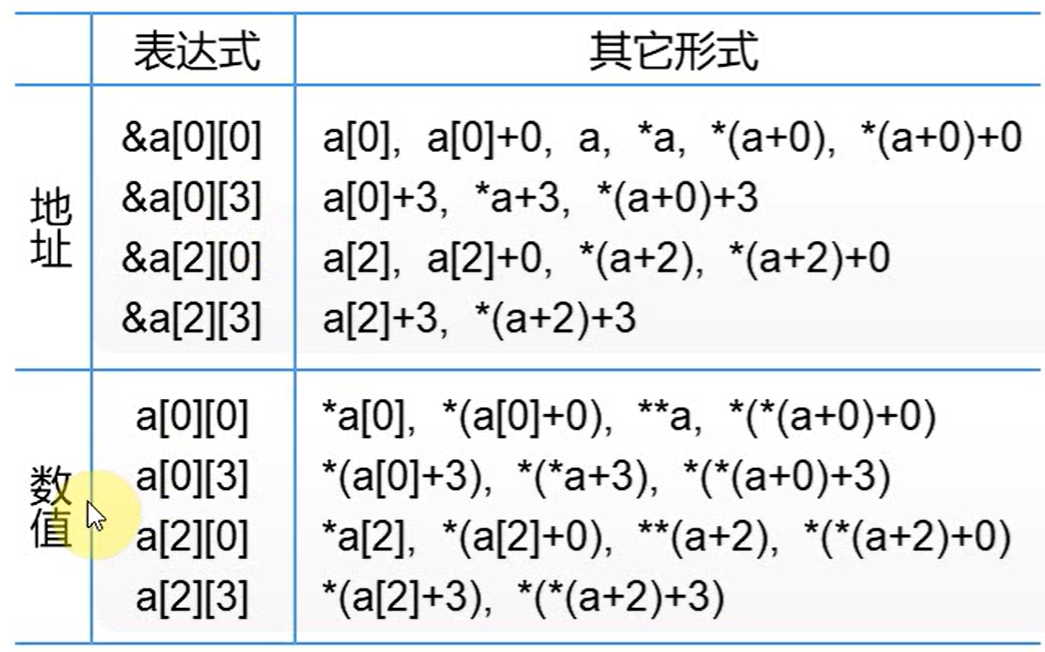
\includegraphics[width=0.4\textwidth]{pic/二维数组地址与值.png}
    \caption{二维数组地址与值}
\end{figure}

\subsubsection{指向数组的指针与元素为指针的数组:}
定义一个指针,指向一维int型数组(长度为2);同时,定义元素为指针的数组(长度为2),语法如下:
\begin{lstlisting}
int (*p)[2];        //定义指针,指向含两个int元素的数组

int *p[2];          //定义数组,数组含两个指针,指针指向int

//因为 [] 运算符的优先级高于 * 运算符,也即int *p[2]等价于int *(p[2])
\end{lstlisting}\par
定义一个指针,指向二维int型数组(大小2*4);同时,定义元素为指向指针的指针的一维数组(长度为2),语法如下:
\begin{lstlisting}
int ((*p)[2])[4];       //定义指针,指向二维int型数组
int (*p)[2][4];         //与上面的定义等价

int **p[2];         //定义数组,元素为指向指针的指针
\end{lstlisting}\par
特别地,如果要定义一个函数,传入的参数为二维数组(大小2*4),这等价于指向一维数组的指针,因此可定义函数为:
\begin{lstlisting}
int function(int (*p)[4], int rows){函数体}   
/*
定义函数,第一个传入参数既可理解为二维数组(大小k*4),也可理解为指向一维数组的指针
(本质是一样的),第二个传入参数为二维数组行数。
*/

\end{lstlisting}
类似地,如果函数要返回一个二维数组,可以定义函数为:
\begin{lstlisting}
int **function(传入参数){函数体}            //定义函数,返回值为两重指针
\end{lstlisting}
\chapter{进阶知识}
\section{字符串及其函数}
\subsubsection{定义字符串:}
\ding{172}\ 字符串常量:用双引号包围字符。\par
\begin{lstlisting}
"I love you!"
\end{lstlisting}
{\color{gray}\small 字符串常量属于静态存储类别(static storage class),这说明定义字符串常量后,该字符串会一直储存在内存中,直到程序结束释放内存。特别地,如果要在字符串内部使用双引号,必须在双引号前面加上一个反斜杠}\par
\ding{173}\ 字符串数组:
\begin{lstlisting}
char a[] = "I love you!";
\end{lstlisting}
    \par
\ding{174}\ 指向字符串的指针:
\begin{lstlisting}
char * a = "I love you!";
const char * a = "I love you!"; // 推荐用法(不要用指针直接指向字符串常量)
\end{lstlisting}\par
{\color{gray}\small 数组形式和指针形式主要的区别是:数组名客观上是指向自身地址的指针常量(其值是自己的地址),作用上是指向首元素地址的指针常量(地址常量),而指针名a是指针变量。}\par
另外,当写下“I love you!”时,实际上“出现”的是一个数组名,数组名的意义见笔记前文,下面代码的输出可以帮助理解:
\begin{lstlisting}
printf("数组名的地址是:%p\n", &"love");
printf("数组名的值是:%p\n", "love");
printf("*数组名的结果是:%c\n", *"love");
printf("*(数组名+2)的结果是:%c\n", *("love" + 2));

数组名的地址是:00007FF7A4A99C10
数组名的值是:00007FF7A4A99C10
*数组名的结果是:l
*(数组名+2)的结果是:v
\end{lstlisting}
\par
\ding{175}\ 字符串数组:下面是一个例子:
\begin{lstlisting}
char * a[2] = { "love","you"};
char (*b)[5] =  "love";       //思考:两种定义有什么不同?
// a是一维数组,含有两个指针元素;b是指向一维数组的指针,此一维数组是字符串。
\end{lstlisting}

\subsubsection{字符串输入:}
\ding{172}\ gets(数组名)函数:gets函数读取整行输入,直至遇到换行符,然后丢弃换行符,储存其余字符,并在这些字符的末尾添加一个结束符使其成为一个字符串。下面是一个例子:
\begin{lstlisting}
char words[80];
gets(words);
\end{lstlisting}
{\color{gray}\small 使用gets函数时,需要确保输入的字符串不超过上限值。如果输入的字符串过长,会导致缓冲区溢出,即多余的字符超出了指定的目标空间。如果这些多余的字符只是占用了尚未使用的内存,就不会立即出现问题;如果它们擦写掉程序中的其他数据,会导致程序异常中止;或者其他更糟糕的情况。}\par
\ding{173}\ fgets(数组名, n)函数:fgets()函数通过第2个参数限制读入的字符数来解决溢出的问题,常同于处理文件。下面是一个例子:
\begin{lstlisting}
char words[20];
fgets(words, 20, stdin);
\end{lstlisting}
{\color{gray}\small 第二个参数的值是n,那么fgets()将读入n-1个字符,或者读到遇到的第一个换行符为止。并且,fgets()读到一个换行符而停止的同时,会把此换行符储存在字符串中,而gets()会丢弃换行符。第三个参数表示输入标准(暂无需了解)。}\par
\ding{174}\ gets\_s(数组名, n)函数:类似fgets,但是gets\_s读到换行符会丢弃它同时停止;且输入超出限定时会进行一些特殊处理并返回空指针。例子略。
{\color{gray}\small 如果gets\_s读到最大字符数都没有读到换行符,会执行以下几步,首先把目标数组中的首字符设置为空字符,读取并丢弃随后的输入直至读到换行符或文件结尾,然后返回空指针。}\par
\ding{175}\ scanf()函数:scanf有两种结束输入的方法。仅控制格式(\%s)时,以空白字符(空行、空格、制表符或换行符)结束输入(不存储空字符)。指定了字段宽度时(\%10s),会在读取到10个字符或读到空白字符时停止。另外,scanf函数返回int 型(表示成功读取并赋值的参数个数)或返回EOF。{\color{gray}\small 在Visual Studio 2022 中是scanf\_s函数。}\par
\ding{176}\ s\_gets()函数:很常用的自定义函数,用于获取用户之前的键盘输入,并将其以字符串形式储存在指定地址。下面是一个例子:
\begin{lstlisting}
void s_gets(char* str, int n) {
    char* result;
    int ch;
    result = fgets(str, n, stdin);
    if (result) {
        while ((ch = getchar()) != '\n' && ch != EOF)
            continue;
    }
    return result;
}
\end{lstlisting}
\subsubsection{字符串输出:}
\ding{172}\ puts(字符串地址)函数:参数为字符串的地址,末尾自动输出换行符。该函数在遇到结束符时停止输出,否则一直输出此后内容直至遇到结束符,所以必须确保是字符串(有结束符)。\par
\ding{173}\ fputs(字符串地址, n)函数:puts的延拓,常用于处理文件输出。\par
\ding{174}\ prinft()函数:最常用,但耗时比前面的长,略。

\subsubsection{字符串函数:}
\ding{172}\ strlen(字符串地址)函数:输入字符串地址(数组名),输出字符串长度(不包含结束符)。\par
\ding{173}\ strcat(字符串1,字符串2)函数:输入两个字符串的地址,将第二个字符串拼接到第一个之后,输出第一个字符串的地址。\par
\ding{174}\ strncat(字符串1,字符串2, n)函数:strcat的延拓,可以指定最大拼接字符数。\par
\ding{175}\ strcmp(字符串1, 字符串2)函数:比较两个字符串的内容,相同则返回0,否则返回非零值(实际上是返回ASCII序号差,字符1减字符2)。{\color{gray}\small strcmp比较字符串而非数组,例如char a[10]和char b[5]都存放了字符串``love'',函数会返回0。}\par
\ding{176}\ strncmp(字符串1, 字符串2, n)函数:strcmp 的延拓,可以指定最大比较字符数。\par
\ding{177}\ strcpy(字符串1, 字符串2)函数:用于将字符串2拷贝到字符串1。{\color{gray}\small 在VS2022中是strcpy\_s(str1,sizeof(str1),str2),返回值为0表示字符串无差异,即复制成功(对ASII码作差)}\par
\ding{178}\ strncpy(字符串1, 字符串2, n)函数:strcpy的延拓。\par
\ding{179}\ sprintf(字符串地址, 数据1, 数据2, ...):把多个数据(可以是字符串、数字等)组合成字符串,但并不打印到显示屏。

\section{存储类别、内存管理}
\subsubsection{作用域:}
\ding{172}\ 块作用域:块是用一对花括号括起来的代码区域。{\color{gray}\small 如函数体,函数中的任意复合语句。}\par
\ding{173}\ 函数作用域:变量在函数内定义,则其作用域为整个函数。\par
\ding{174}\ 函数原型作用域:即形参的作用域,从形参定义处到函数原型全部结束。\par
\ding{175}\ 文件作用域:在文件顶部用static定义的变量或函数,作用域为整个文件。\par
\ding{176}\ 全局作用域:在文件顶部用定义的变量或函数,可以在多文件程序中使用。{\color{gray}\small 如果外部变量定义在一个文件中,那么其他文件在使用该变量之前必须用 extern 声明它。函数也有存储类别,可以是外部函数(默认,多文件可用)或静态函数(static,本文件可用)。}
\subsubsection{存储期:}
\ding{172}\ 自动存储期:程序进入块时,为变量分配内存;退出这个块时,释放所分配的内存。{\color{gray}\small 块作用域的变量通常都具有自动存储期。块作用域变量也能具有静态存储期,从而在不同的函数之间进行调用。创建这样的变量只需在块中的声明前加上static。}\par
\ding{173}\ 线程存储期:用于并发程序设计,从被声明时到线程结束一直存在。\par
\ding{174}\ 静态存储期:在程序的执行期间一直存在。{\color{gray}\small 文件作用域、文件作用域变量具有静态存储期。}\par

\begin{table}[H]
    \centering
    \caption{C语言六种存储类别说明符}
    \begin{tabular}{cc}
        \toprule
        说明符 & 作用\\
        \hline
        auto & 默认存储类别(不常用)\\
        register & 将局部变量存储在寄存器中(不常用)\\
        static & 改变作用域(文件头处,文件 to 全局)、改变存储期(块内,自动 to 静态)\\
        extern & 声明在其他文件中定义的全局变量或函数\\
        \_Thread\_local & 指定变量为线程存储期\\
        typedef & 创建类型别名\\
        \bottomrule
    \end{tabular}
\end{table}
\subsubsection{分配并释放内存:}
\ding{172}\ malloc( n*sizeof() )函数:分配连续内存块,返回 viod* (即通用指针,配合类型转换使用),分配失败时返回空指针NULL。下面是一个例子:
\begin{lstlisting}
#include <stdio.h>
#include <stdlib.h>     //提供malloc()和free()
void main() {
    int n = 0;
    int * p = NULL;
    scanf("%d",&n);
    p = (int*) malloc( n*sizeof(double) )   //分配n个double类型的内存
    if(p == NULL){printf("内存分配失败!\n");}
    else{printf("内存分配成功,进入下一步\n");}
    printf("分配的内存可以释放了\n");
    free(p);
}
\end{lstlisting}
{\color{gray}\small 应坚持使用强制类型转换,以提高代码的可读性、可延展性。另外,一定勿忘释放内存,也不要忘了\#include <stdlib.h>。另外,使用动态内存通常比使用栈内存(自动变量所占据的内存)慢,因此不需要动态时更建议使用栈内存。}\par
\ding{173}\ calloc( n, sizeof() ):类似malloc,但自动把内存中所有位都设置为0。\par
\ding{174}\ free():释放内存。\par

\subsubsection{类型限定符:}
\ding{172}\ const: 以const关键字声明的对象,其值不能被程序修改。\par
\ding{173}\ volatile: 告知计算机,代理(而不是程序)可以改变该变量的值。\par
\ding{174}\ restrict: 只能用于指针,允许编译器优化某部分代码以更好地支持计算。 \par
\ding{175}\ \_Atomic: 当一个线程对一个原子类型的对象执行原子操作时,其他线程不能访问该对象。

\section{文件输入/输出}
\subsubsection{文件函数:}
常用的文件函数有fopen, fclose; getc, fgets, fscanf; putc, fputs,  fprintf; fread, fwrite 等。\par
\ding{172}\  fopen("filename", mode):打开文件,打开成功则返回int 0,否则返回NULL。{\color{gray}\ 常见的mode有"r", "w", "a", "r+", "w+", "a+"}\par
\ding{173}\  fclose(FILE*):关闭文件,关闭成功则返回int 0,否则返回EOF。\par

\ding{174}\ getc(FILE*)或fgetc(FILE*): 读取当前位置字符,并将位置+1(可理解为光标位置+1)。\par
\ding{175}\ putc(int\_Character ,FILE*)或fputc(int\_Character, FILE*): 输入字符、数字等,int\_Character为字符的ASII值(也可以直接传char,如‘r’)。\par
下面是\ding{172}\ding{173}\ding{174}\ding{175}的一个例子:
\begin{lstlisting}
FILE* pf = fopen("C:\\Users\\13081\\Desktop\\c_learning.txt", "r+");
if (pf == NULL){perror("fopen");}
else{ printf("文件打开成功\n"); }
int e = 5;
if (pf!= NULL){ 
    printf("%c\n", getc(pf)); printf("%c\n", getc(pf));		//get并输出两个字符
    putc('w', pf); 	putc('\n', pf);	putc('h', pf); e = fclose(pf); printf("已添加数据\n");  //输入三个字符
}
if (e == EOF) { perror("fclose"); }
else{ printf("文件关闭成功\n");  printf("e为%d", e);} 
\end{lstlisting}\par
\ding{176}\ fgets(char*, int, FILE*): get并return字符(用字符数组接受)。\par
\ding{177}\ fputs(const char*, FILE*): 输入字符串。\par
下面是\ding{176}\ding{177}的例子:
\begin{lstlisting}
FILE* pf = fopen("C:\\Users\\13081\\Desktop\\c_learning.txt", "w+");
if (pf == NULL){perror("fopen");}
else{ printf("文件打开成功\n"); }
int e = 5;
if (pf!= NULL){ 
    fputs("but she don't love me", pf); printf("fputs添加成功\n");		//fputs
    fseek(pf, 0, SEEK_SET);			//重置光标至开头
    char str[100]; fgets(str, 100, pf); printf("get到str为%s\n", str);		//fgets
    e = fclose(pf);		//关闭文件
}
if (e == EOF) { perror("fclose"); }
else{ printf("文件关闭成功\n");  printf("e为%d", e);}
\end{lstlisting}
\par
\ding{178}\ fscanf( FILE*, const char* format, ...): 参数2是将要读取的数据格式(和scanf函数一样有\%d,\%x,\%c,\%s等等格式类型),参数3是储存数据的地址,将读取到的数据储存在目标地址。\par
\ding{179}\ fprintf( FILE*, const char* format, ...): 参数2是格式,参数3是要输出的数据。\par

\ding{180}\ fwrite( const void*, size\_t size, int num, FILE* ): 参数1是要传入的数据(如数组),参数2是sizeof(类型)返回的值,参数3是数据个数,参数4是文件指针。\par
\ding{181}\ fread( void*, size\_t size, int num, FILE* ): 参数1是储存数据的地址,参数2是sizeof(类型)返回的值,参数3是数据个数,参数4是文件指针。{\color{gray}\small fread,fwrite函数}\par
\subsubsection{文件读写光标位置}
\ding{172}\ ftell():返回文件指针相对于起始位置的偏移量:\par
\ding{173}\ fseek( FILE*, long int, mode): 移动光标,参数1是文件,参数2是偏移量,参数3是模式(决定偏移起点),SEEK\_SET为文件开始处,SEEK\_CUT为当前光标位置,SEEK\_END为文件结尾处。下面是一个例子:
\begin{lstlisting}
fseek(fp, -10L, SEEK_END); // 从文件结尾处回退10个字节
\end{lstlisting}
\par
\ding{174}\ rewind( FILE* ):将所传入的文件指针设置指向文件初始位置。
{\color{gray}\small 数据在内存中以二进制的形式存储,如果不加转换的输出到外存(磁盘等),就是二进制文件。在外存中以ASCII字符的形式存储的文件就是文本文件。}
\subsubsection{判断文件结尾还是出错:}
\ding{172}\ feof( FILE* ):判断文件为何读取结束,若因到达文件结尾返回0,否则返回非零值。\par
\ding{173}\ feof( FILE* ):判断文件为何读取结束,若因出错而结束,返回非零值。

\section{结构、联合、枚举与自定义类型}
\subsubsection{结构体模版、结构体变量:}
结构体可以封装一些属性,是一种数据类型,=,也就是说可以用它来定义变量。下面是一个例子:
\begin{lstlisting}
#include <stdio.h>

struct Birthdate {
    int year;
    int month;
    int day;
};
struct Student {     // 定义名为“Student”的结构模版
    char id[8];     // 结构体内各种数据
    char name[8];
    char sex[4];
    int age;
    struct Birthdate birthday;
};              // 一定别忘了分号

int main() {
    struct Student dy = { "130810", "Ding Yi", "man", 18, 2004, 9, 15 };
    printf("成员id: %s\n成员name:%s\n成员性别:%s\n成员年龄:%d\n成员生日:%d.%d.%d\n\n", dy.id, dy.name, dy.sex, dy.age, dy.birthday.year, dy.birthday.month, dy.birthday.day);
    dy.age = 80;
    printf("成员id: %s\n成员name:%s\n成员性别:%s\n成员年龄:%d\n成员生日:%d.%d.%d\n\n", dy.id, dy.name, dy.sex, dy.age, dy.birthday.year, dy.birthday.month, dy.birthday.day);
}
\end{lstlisting}
{\color{gray}\small 定义结构体变量也可以使用匿名结构(没有给定义的结构体起名字),详略。}
\subsubsection{结构体指针、结构体数组:}
使用结构体指针时,可按常规用(*p).name,也可使用p->name。\par
{\color{gray}\small .的优先级高于*,(*p)两边括号不能少,->为指向符。在函数需要传入一个结构体参数时,建议传入结构体指针而非结构体变量(这在内存中更高效)。另外,如果需要防止结构变量中的数据被改变,可以使用 const struct Student *p,此语句的实际意义等价于 (const struct Student) (*p) ,即p指向的内容是一个 const struct Student 。}\par
结构体数组,是指数组中的每一个元素都是一个结构体类型。详略。
\subsubsection{结构体在内存中的存储方式及大小:}
三个规则:\par
\ding{172}\ 结构体变量的首地址,必须是结构体变量的“最大基本数据类型成员所占字节数”的整数倍。\par
\ding{173}\ 结构体变量中的每个成员相对于结构体首地址的偏移量,都是该成员基本数据类型所占字节数的整数倍。\par
\ding{174}\ 结构体变量的总大小,为结构体变量中“最大基本数据类型成员所占字节”的整数倍。\par
下面是一个例子:
\begin{figure}[H]
    \centering
    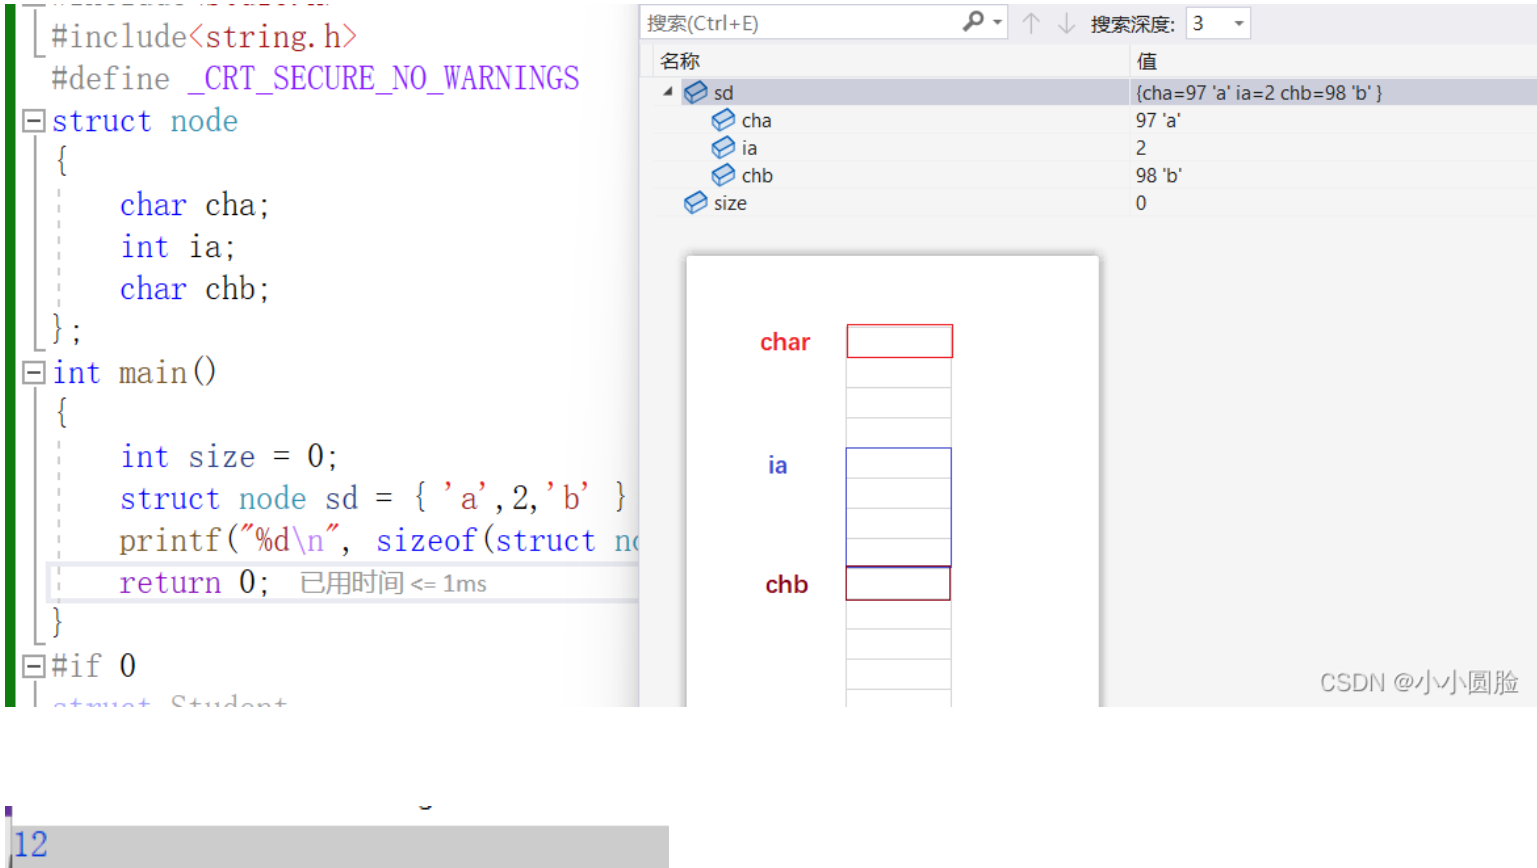
\includegraphics[width=\textwidth]{pic/结构体.png}
    \caption{结构体示例}
\end{figure}
\subsubsection{伸缩型数组成员:}
详见: https://blog.csdn.net/qq\_43296898/article/details/88870073
\subsubsection{复合字面量:}
可用于数组、结构、联合体等。例如,可以使用复合字面量创建一个数组同时创建指向此数组的指针,下面是一个例子:
\begin{lstlisting}
char* p = (char[]){"love"};
printf("%s", p);
\end{lstlisting}
\subsubsection{联合:}
联合是一种特殊的自定义类型,能在同一个内存空间中储存不同的数据类型(不是同时)。联合的定义类似结果,下面是一个例子:
\begin{lstlisting}
union xyz {
    int n;
    double d;
    char c;
};
union xyz fit;     // xyz类型的联合变量
union xyz myarray[10]; // 内含10个联合变量的数组
union xyz *p; // 指向xyz联合变量的指针

fit.n = 23; //把 23 储存在 fit,占4字节
fit.d = 2.0; // 清除23,储存 2.0,占8字节
fit.c = 'h'; // 清除2.0,储存h,占1字节
\end{lstlisting}
\subsubsection{枚举:}
枚举类型和宏定义类似,只有细微区别,宏运行是在预处理阶段完成的,枚举类型是在与编译阶段完成的。详见: https://blog.csdn.net/weixin\_73233099/article/details/128761416
\subsubsection{typedef类型别名:}
typedef可为已有的数据类型取一个新的名字(创建新标识符)。下面是一个例子:
\begin{lstlisting}
# include <stdio.h> 
typedef struct Student {
    char name[100];
    int age;
    char sex;
    double score;
} STU;
 
int main (void) {
    struct Student stu1 = {"Cyan", 21, 'M', 425};
    STU stu2 = {"Rain", 19, 'F', 444};
 
    STU * pst1 = &stu1;
    STU * pst2 = &stu2;
    
    printf("第一个学生stu1的信息如下:\n");
    printf("name = %s\t", stu1.name);
    printf("age = %d\t", stu1.age);
    printf("sex = %c\t\t", stu1.sex);
    printf("score = %.2lf\t", stu1.score);
    printf("\n===========================\n");

    printf("第二个学生stu2的信息如下:\n");
    printf("name = %s\t", pst2->name);
    printf("age = %d\t", pst2->age);
    printf("sex = %c\t\t", pst2->sex);
    printf("score = %.2lf\t", pst2->score);
    printf("\n===========================\n");

    return 0;
}
\end{lstlisting}
\subsubsection{函数指针:}
https://blog.csdn.net/u010280075/article/details/88914424

\section{位操作:}
\subsubsection{进制及其转换:}
\begin{table}[H]
    \centering
    \caption{半字节整数转换}
    \begin{tabular}{ccccccccc}
    \toprule
    二进制 & 0000 & 0001 & 0010 & 0011 & 0100 & 0101 & 0110 & 0111\\
    十进制 & 0 & 1 & 2 & 3 & 4 & 5 & 6 & 7\\
    十六进制 & 0 & 1 & 2 & 3 & 4 & 5 & 6 & 7\\
    \hline
    二进制& 1000 & 1001 & 1010 & 1011 & 1100 & 1101 & 1110 & 1111\\
    十进制& 8 & 9 & 10 & 11 & 12 & 13 & 14 & 15\\
    十六进制& 8 & 9 & A & B & C & D & E & F\\
    \bottomrule
    \end{tabular}
    \end{table}
\newpage
\nocite{*}
\bibliography{re}
\addcontentsline{toc}{chapter}{参考文献}


\newpage
\appendix
\addcontentsline{toc}{chapter}{附录}
\titleformat{\section}{\large\centering\bfseries}{附录\thesection}{1em}{}
\titleformat{\subsection}{\normalsize\bfseries}{\thesubsection}{1em}{}

\section{常用功能}
\begin{longtable}[H]{cc}
    \caption{\textbf{Visual Studio 2022 常用快捷键}}\\
    \toprule
    快捷键 & 功能\\
    \midrule
    \endfirsthead
    % 这里是表格内容
    \bottomrule
    \endfoot

    \toprule
    \multicolumn{2}{c}{\textbf{续上表}}\\
    \midrule
    快捷键 & 功能\\
    \midrule
    \endhead
    % 这里是表格内容
    \bottomrule
    \endlastfoot
    Ctrl + K + D & 对齐代码\\
    Ctrl+K+C & 注释\\
    Ctrl+K+U & 取消注释\\
    Tab & 增加缩进\\
    Shift +Tab & 减少缩进\\
    Ctrl + J & 弹出智能提示\\
 \end{longtable}

 \begin{table}[H]
    \centering
    \caption{常用函数库}
    \begin{tabular}{cc} 
    \toprule
    数学函数库  & math.h     \\
    字符函数库  & ctype.h    \\
    字符串函数库 & string.h  \\
    \bottomrule
    \end{tabular}
\end{table}


\end{document}

